% -*- coding: utf-8 -*-
%!TEX root = ../book.tex

\cleardoublepage
\plainifnotempty

\chapter{クラウド時代のDNS}
\begin{flushright}
suu-g (@suu\_g)
\end{flushright}

%\section{Welcome to DNS world}
\lettrine{ヰ}
ンターネットが始まってから20年、ARPANETから数えると40年以上。
インターネットはここ10年ほどで一気に生活に不可欠のものとなりました。
そんなインターネットを支える基礎技術の一つがDNSです。

そのDNSを取り巻く状況ですが、今年は随分と熱い一年間でした。
普通のソフトウェア屋さんにとってDNSとは使うものであって
それ以外ではないのでしょうから、こちらの世界のニュースについては
あまり確認されていないことと思います。
今年は、どんな問題が起きたのでしょうか?振り返ってみましょう。
\begin{itemize}
  \item (日本)児童ポルノに関するDNSブロッキング立法・ISPにおける運用が開始
  \item SOPAにGo Daddyが賛成を表明するも1日で撤回
  \item SOPAに反対を表明するためWikipediaが24時間閉鎖する
  \item SOPAに反対を表明してAnonymousがOperation Blackoutを表明
  \item v6-v4フォールバック問題の対策法としてAAAAフィルタリングが検討される
  \item Google, AAAAフィルタを導入している可能性のあるDNSサーバに対してAAAAレコードを回答しない運用を宣言
  \item Ghost Domain問題の発表
  \item ニフティクラウドのDNS障害問題
  \item GMOクラウドのDNSで謎の障害がある
  \item さくらのDNSに(サブ)ドメインジャッキングが可能な脆弱性が発覚
  \item JPRSがあらためてコンテンツサーバとキャッシュサーバの兼用の危険性を告知
  \item BIND, 長さ0のRDATAにより異常終了する脆弱性(重複をお許しください)
  \item お名前.com、忍者ツールズのNSレコードを規約に基づき変更
  \item 今年の夏のDNS祭りはBINDではなくNSD
\end{itemize}

問題に限定しなければ他にも、DNSSEC.jpが活動を終了したり、
gTLDの申請があったりと、今年は本当に色々なことがありました。

DNSの最初のRFC 1034, 1035 が出たのは1987年でしたが、それから25年
経過し、「クラウド」時代と言われる今でもなお起こり続ける
DNS障害。その原因とは一体、何なのでしょうか?
この記事では、DNSを一種の分散システムと考えて、それを
ソフトウェアっぽい視点から見ていくことで、
その問題の一端を解き明かします。 
解き明かすと思う。解き明かすんじゃないかな。まあ、ちょっと覚悟してください。



\section{DNSの正常系}
\subsection{DNSとぼくらの世界}

\begin{figure}[hbt]
\begin{minipage}{0.3\hsize}
{\scriptsize
\begin{verbatim}
Query

{
  Header: {
    ID,
    is_query,
    Flags: {
      AA: 1 or 0,
      TC: 1 or 0,
      RD: 1 or 0,
      RA: 1 or 0,
    }
  },
  Query: [{
    Name: "www.example.jp.",
    Type: "AAAA",
    Class: "IN",
  }],
  Answer: [],
  Authoritative: [],
  Additional: []
}
\end{verbatim}
}
\end{minipage}
\begin{minipage}{0.3\hsize}
{\scriptsize
\begin{verbatim}
Answer

{
  Header: { ... },
  Query: [{
    Name: "www.example.jp.",
    Type: "AAAA",
    Class: "IN",
  }],
  Answer: [{
    Name: "www.example.jp.",
    Type: "AAAA",
    Class: "IN",
    TTL: 86400,
    RData: "2001:DB8::163"
  }],
  Authoritative: [],
  Additional: []
}
\end{verbatim}
}
\end{minipage}
\begin{minipage}{0.3\hsize}
{\scriptsize
\begin{verbatim}
Answer

{
  Header: { ... },
  Query: [{ ... }],
  Answer: [],
  Authoritative: [],
    Name: "example.jp.",
    Type: "NS",
    Class: "IN",
    TTL: 86400,
    RData: "ns.example.jp"
  Additional: []
    Name: "ns.example.jp",
    Type: "AAAA",
    Class: "IN",
    TTL: 86400,
    RData: "2001:DB8::160"
}
\end{verbatim}
}
\end{minipage}
\caption{
DNSパケットのJSON風表記
}
\label{jsondns}
\end{figure}


DNSのパケットフォーマットは、RFC1034
\footnote{http://www.ietf.org/rfc/rfc1034.txt Section 3-7}
,1035 
\footnote{http://www.ietf.org/rfc/rfc1034.txt Section 4-1}
に載っている通りです。
4つのセクションがあり、それぞれQuery, Answer, Authority,
それからAdditionalと呼ばれています。
これをJSON風に書くと、図\ref{jsondns}のようになってます。
(正確には、DNSSECやEDNS0対応等でフラグはもう幾つかある)
読者の皆様におかれましてはこのパケットの意味を判断しようとしてくれると
期待しますが、勘の良い人だと、このプロトコルのもつ怪しさをなんとなく
感じ取ったかも知れません。

さて、このようなパケットを元にして、DNSというシステムは成り立っています。
このパケットを用いて Paul Vixie らが作ろうとしたのが、巨大な名前空間の木です。
そして、その木をデータベースとしてユーザから参照できるようにした。それが
DNSというシステムです。あ、ご存知ですよね。すいません。でも大事なこと
なんで。

ここでnoteしておきたいのが、DNSプロトコルが作られた当時の時代情勢です。
DNSは、/etc/hostsからの移行のひとつの可能性として生まれていたわけですが、
その時代が今とは違っていて、例えばDNSでちょっと間違いが起こったとしても、
それは手動で直していれば良かった。今じゃ警察沙汰だもん。

もっとも、DNSに関しては今でも法的にきちんとしているとは言い難いところです。
DNSでのブロッキングの効果を法律で認めているわりには、JPRSが電気通信事業者
というわけでもありませんし。このあたりは、そろそろ本格的に議論されるべき
話ですよね。

さて話は戻ります。いま当時の時代情勢を取り上げたのは、DNSという
分散システムが、設計段階から「異なる管理者同士で」ひとつの巨大な名前空間を
管理するように作られている、ということを再認識したかったからです。
各管理者が責任を持つ名前空間の範囲をゾーンと呼び、その空間の管理を他の人に
任せることを委譲と呼んでいる。そういう信頼関係となっています。
それらを前提として、内容に入って行きましょう。


\subsection { 基本動作 }

\begin{figure}[b]
\centering
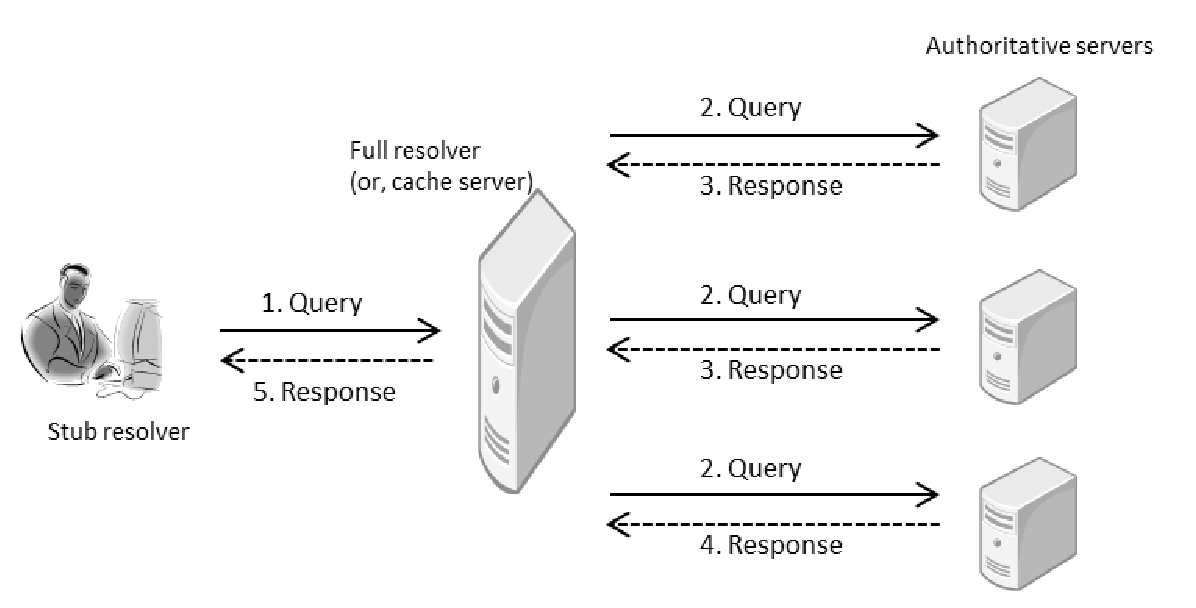
\includegraphics[width=\textwidth]{./suu-g/zuuu.eps}
\caption{DNSにおいてやりとりされるパケット}
\label{packet}
\end{figure}

DNSの正常系は、先に示しました4つのセクションと5つのフラグを使い、
おおよそ次の5種類のパケットを用います。
{\small
\begin{enumerate}
  \item Query (recursive)
  \item Query (not recursive)
  \item Response (Authoritative, with glue record in additional section)
  \item Response (with Answer)
  \item Response (against recursive query)
\end{enumerate}
}

ユーザがキャッシュサーバに対して問い合わせを行い、そのキャッシュサーバ
がユーザの代わりにイテラティブにクエリを発行するときのパケットは、
それぞれ図\ref{packet}のようになります。
キャッシュサーバがキャッシュを持ったあとは、1と5のパケットのみの
やりとりとなります。ここまでは皆様ご存じですねー。
また、このキャッシュサーバがコンテンツサーバも兼ねている場合、
キャッシュサーバから直接4の、権威あるレスポンスが返ってくることになります。
なお、権威のある回答は通常のキャッシュと比較して優先されるべき
ものということになっています
\footnote{http://www.ietf.org/rfc/rfc2181.txt}
が、スタブリゾルバではどちらも信用するので同じものとして扱われます。

正常系としては、こんなところでしょう。この決め事によって、
ルートサーバを頂点とする綺麗なツリー構造が世界に作れます。


\section { DNSの異常系 }
以上のようなDNSですが、問題が山積みです。これはどう考えても
プロトコルが悪いのです。DNSのプロトコルがこんなに狂っているはずがない。

\subsection{ Lame Delegation }
これは基本ですね。 要は、上位のサーバでの正しくない設定です。
構造的には、 Visaドメイン問題 
\footnote{http://www.e-ontap.com/summary/}
と言われているものもこれのうちのひとつですね。
Lame delegationのあるドメインは、最悪の場合は即日乗っ取りが可能です。
基本ったら最強ね。


\subsection{ 浸透さんって幽霊じゃね? }

DNSの設定変更や引っ越しをしたときに、その結果が「浸透」
するのを待たなければいけない…というのは有名な嘘です。
DNSはキャッシュを持つだけなのだから、そんな現象は存在しない。
…そう言われていたのですが、キャッシュに許容された以上の間、
キャッシュが保持されてしまう問題が実在したことがわかりました。
これが "Ghost Domain" 
\footnote{www.isc.org/files/imce/ghostdomain\_camera.pdf}
問題(日本語で「幽霊ドメイン」問題)です。 
その原因は、複数のサーバソフトウェアに同様に存在した実装不具合でした。

詳細な問題内容については、DNSOpsの資料 
\footnote{http://dnsops.jp/bof/20120425/20120425-DNSOPS.jp-BoF\_Ghost\_Domain\_Names\_v02.pdf}
や「Geekなぺーじ」
\footnote{http://www.geekpage.jp/blog/?id=2012/3/21/1} に詳しい
のでそちらをご覧ください。

ソフトウェア的に考えたときに問題なのは、古いキャッシュ
が残存して昔のサーバへ問い合わせを続けるということ、
それから、問い合わせを続けていると古いキャッシュがexpire
しないという実装バグがあったということ。そして最後に、
本来のDNSのツリーから外れたコンテンツサーバが、レコードを
消さずに残しているために、昔のレコードをいつまでも返し続ける
場合があるということ。この三点です。

本来の信頼関係から外れたところのデータが有効性を持ってしまい、
おまけにその状態を意図的に作り出せる、という状態ですね。
このような問題が今年までバグとして存在し続けていたわけです。

システムとして考えると、キャッシュをTTL分保持することは
至極もっともなようですが、信頼関係のツリーまで含めてキャッシュすると
いうことは、非常に責任が大きい行為でした。
今回のように、「なぜかキャッシュが消えない」という
異常事態になったとき、影響が大きくなります。
当然、負荷とのトレードオフですけどね。


\subsection{ サブドメインジャッキング問題 }
2011年6月、さくらのDNSサービスにおいて、一時的にサブドメイン
ジャッキングが可能になっていた問題が発覚しました。
これは、 example.jp ドメインが登録されていたとしても、別のユーザに
よって自由に www.example.jp ドメインを作成できてしまった、という
問題です
\footnote{さくらはたまたま注目を浴びただけで、問題を抱えたサービス
プロバイダは他にもたくさんある…が、その話はまた今度}
。 これは、DNSの本質的な問題を幾つか激しく突いています。

ひとつには、DNSの作成しているツリーが理想的なものではないこと。
理想的には権威サーバはすべて異なるサーバであるべきですが、
現実的には相乗りが発生します。
同じ階層のドメインやゾーンの相乗りならさほど問題はありませんが、
親子ゾーン・孫ゾーンが同じサーバ上に乗ると、
サーバ同士の依存関係が崩れてしまいます。
結果、「正しい依存関係」を順番に辿って回答にたどり着く、という
DNSの基本動作から外れることになり、鼻から悪魔が出ます。

ふたつめとして、ゾーンと言う概念が、プロトコルや実装とかけ離れて
しまっているという点があります。
ドメインのデリミタはドットですが、ドットがあったからと言って
ゾーンの切れ目となっているかどうかは不明です。
example.jp ゾーンを他へ委譲したサーバ上で www.example.jp のAレコードの
登録は(ソフトウェア的に)できますし、www.example.jpを問い合わせた
ときにどちらが返って来るかは実装依存になってしまっています。

最後に、フルリゾルバがどのコンテンツサーバにも同じクエリを投げる、
というプロトコルの怪しさがあります。
これは、どこでゾーンが分かれるかが問い合わせを行うまでは
キャッシュサーバには知ることができない、ということとは符合します。
しかし、キャッシュサーバはゾーンの別れ方について、知らないでは済まされない。
問い合わせを行ったキャッシュサーバは、即座にその結果をキャッシュします。
このキャッシュを正しく行うためには、「現在問い合わせている先がどのゾーンの
Authorityを持っているか」という情報が必須です。
したがってキャッシュサーバは問い合わせの際に状態を持っています。
状態を持っているのに、その状態を利用して問い合わせ内容を変更しなかったこと。
これが大罪です。
もしも問い合わせがゾーンごとに行われていれば、子ゾーンについて問い合わせて
いるところで孫ゾーン情報が返ってきたり、あるいはAレコード問い合わせ
に対して謎のNSレコードをキャッシュさせられたりすることは無かったでしょう。
どう見てもプロトコル上の脆弱性です。本当にありがとうございました。

これらの問題点を合わせて起こった問題が、このサブドメインジャッキング問題です。
「DNSサーバの相乗りという業務形態自体が、プロトコルとの相性が悪いのではないか」
と言った方がいましたが、 その意味が分かるのではないでしょうか。


\subsection{ キャッシュ兼用サーバ }
コンテンツ・キャッシュ兼用サーバはしばしば問題と言われます。
先に示したような、自由に偽ドメインを入れられるコンテンツサーバを
フルリゾルバとして使用するのは、 自分のホストの /etc/hosts の書き換え権を
他人に委ねているようなものだ、というのはお分かりいただけるかと思います。

さて、ソフトウェア的に見た時に、キャッシュ兼用サーバに潜むDNSの問題は
というと…、これは優先順位の問題があります。
AuthoritativeなサーバからのAnswerセクションは、他のどのレコードよりも
優先されるべきだとRFC2181にあります。が、毒入れの可能性を考えたときに
もっとも危険性が高いのも、このAuthoritativeなAnswerセクションです。
本来信頼性が最高レベルのものが一番信用できなくなるのは、プロトコルとして
崩壊していますね。わぁい崩壊。


\section{まとめ}
以上に挙げた問題は、この「クラウド」な一年間で実際に「クラウド」な
業者のもとで起き、社会的に影響を与えたものです。
DNSの問題の多くはそのプロトコルへの不理解によるものですが、
そういうヒューマンエラーが起きやすいような仕組みが、DNSには備わっています。
皆様方におかれましては、このDNSという「想定外に利用されてしまった」
プロトコルの問題を他山の石とし、これからのクラウドちっくな分散システムの
開発にぜひ活かしていただければ、この記事のタイトルが救われるというものです。

以上、タイトル詐欺の記事でした。

